%-------------------------------------------------------------------------------
% Part: INTERFACE
%-------------------------------------------------------------------------------
\part{INTERFACE}


%-------------------------------------------------------------------------------
% Chapter: Overview
%-------------------------------------------------------------------------------
\chapter{Overview}
\label{cha:overview}

\texttt{INTERFACE} is the sub-cluster of syndication with all the
classes a developer needs to use the library. There are classes to
read into and write from a \texttt{FEED}, a \texttt{FEED\_MANAGER} to
administrate a list of \texttt{FEED}s, and a factory class which makes
it easy to create all necessary objects.

See figure \ref{fig:interface} for an overview of the cluster.

\begin{figure}[htbp]
  \centering
  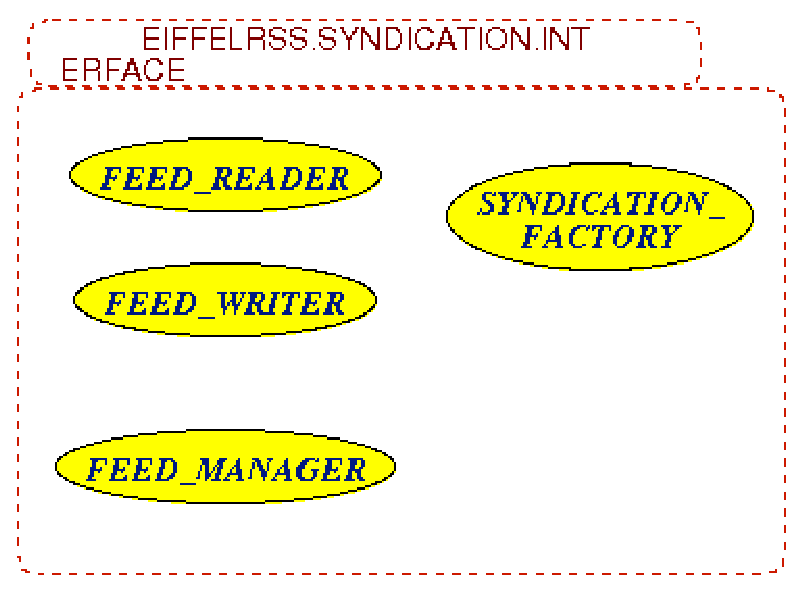
\includegraphics[scale=.6]{./figures/EIFFELRSS_SYNDICATION_INTERFACE}
  \caption{BON diagram of cluster \texttt{INTERFACE}}
  \label{fig:interface}
\end{figure}


%-------------------------------------------------------------------------------
% Chapter: Class SYNDICATION_FACTORY
%-------------------------------------------------------------------------------
\chapter{Class SYNDICATION\_FACTORY}
\label{cha:syndiction-factory}


\section{Overview}
\label{sec:syndication-factory-overview}

\texttt{SYNDICATION\_FACTORY} provides an easy way to create objects
of classes from the cluster \texttt{SYNDICATION}.


\section{Usage}
\label{sec:syndication-factory-usage}

\begin{lstlisting}[language=Eiffel]
class USAGE_EXAMPLE

create 
  make

feature -- Initialization

  make is
      -- Creation procedure.
    do      
      create syndication

      feed := syndication.new_feed ("EiffelRSS", create {HTTP_URL}.make ("http://eiffelrss.berlios.de/"), "EiffelRSS news")

      item := syndication.new_item (channel, "Version 23 released!", create {HTTP_URL}.make ("http://eiffelrss.berlios.de/Main/News"), "Version 23 of EiffelRSS got release today. Happy syndicating!")

      feed.add_item (item)
    end
    
feature -- Arguments

  syndication: SYNDICATION_FACTORY
      -- Syndication factory object

  feed: FEED
      -- Feed object
      
  item: ITEM
      -- Item object
  
end -- class USAGE_EXAMPLE
\end{lstlisting}


\section{Features}
\label{sec:syndication-factory-features}


\subsection{READER factory}
\label{sec:syndication-factory-reader}

\subsubsection{new\_reader\_from\_url }

\begin{lstlisting}[language=Eiffel]
new_reader_from_url (a_url: STRING): FEED_READER
  -- Create with `a_url' as source of feed
\end{lstlisting}


\subsection{WRITER factory}
\label{sec:syndication-factory-writer}

\subsubsection{new\_writer\_from\_feed}

\begin{lstlisting}[language=Eiffel]
new_writer_from_feed (a_feed: FEED): FEED_WRITER
  -- Create a writer object for the feed `a_feed'
\end{lstlisting}


\subsection{FEED\_MANAGER factory}
\label{sec:syndication-factory-feed-manager}

\subsubsection{new\_feed\_manager}

\begin{lstlisting}[language=Eiffel]
new_feed_manager: FEED_MANAGER
  -- Create a new feed manager with default refresh period `30'
\end{lstlisting}


\subsubsection{new\_feed\_manager\_custom}

\begin{lstlisting}[language=Eiffel]
new_feed_manager_custom (a_refresh_period: INTEGER): FEED_MANAGER
  -- Create a new feed manager with default refresh period `a_refresh_period'
\end{lstlisting}


\subsection{FEED factory}
\label{sec:syndication-factory-feed}

\subsubsection{new\_feed}

\begin{lstlisting}[language=Eiffel]
new_feed (a_title: STRING; a_link: URL; a_description: STRING): FEED
  --  Create a feed with title, link and description
\end{lstlisting}


\subsubsection{new\_feed\_from\_channel}

\begin{lstlisting}[language=Eiffel]
new_feed_from_channel (a_channel: CHANNEL): FEED
  -- Create a new feed from an existing channel
\end{lstlisting}


\subsection{CHANNEL factory}
\label{sec:syndication-factory-channel}

\subsubsection{new\_channel}

\begin{lstlisting}[language=Eiffel]
new_channel (a_title: STRING; a_link: URL; a_description: STRING): CHANNEL
  --  Create a channel with title, link and description
\end{lstlisting}


\subsubsection{new\_channel\_cloud}

\begin{lstlisting}[language=Eiffel]
new_channel_cloud (a_domain: STRING; a_port: INTEGER; a_path: STRING; a_register_procedure: STRING; a_protocol: STRING): CHANNEL_CLOUD
  -- Create a channel cloud with domain, port, path, register procedure and protocol
\end{lstlisting}


\subsubsection{new\_channel\_image}

\begin{lstlisting}[language=Eiffel]
new_channel_image (a_url: URL; a_title: STRING; a_link: URL): CHANNEL_IMAGE
  -- Create a channel image with URL, title, and link
\end{lstlisting}


\subsubsection{new\_channel\_text\_input}

\begin{lstlisting}[language=Eiffel]
new_channel_text_input (a_title: STRING; a_description: STRING; a_name: STRING; a_link: URL): CHANNEL_TEXT_INPUT
  -- Create a channel text input with title, description, name and link
\end{lstlisting}


\subsection{ITEM factory}
\label{sec:syndication-factory-item}

\subsubsection{new\_item}

\begin{lstlisting}[language=Eiffel]
new_item (a_channel: CHANNEL; a_title: STRING; a_link: URL; a_description: STRING): ITEM
  -- Create an item with title, link and description
\end{lstlisting}


\subsubsection{new\_item\_with\_title}

\begin{lstlisting}[language=Eiffel]
new_item_with_title (a_channel: CHANNEL; a_title: STRING): ITEM
  -- Create an item with title
\end{lstlisting}


\subsubsection{new\_item\_with\_description}

\begin{lstlisting}[language=Eiffel]
new_item_with_description (a_channel: CHANNEL; a_description: STRING): ITEM
  -- Create an item with description
\end{lstlisting}


\subsubsection{new\_item\_enclosure}

\begin{lstlisting}[language=Eiffel]
new_item_enclosure (a_url: URL; a_length: INTEGER; a_type: STRING): ITEM_ENCLOSURE
  -- Create an item enclosure
\end{lstlisting}


\subsubsection{new\_item\_guid}

\begin{lstlisting}[language=Eiffel]
new_item_guid (a_guid: STRING): ITEM_GUID
  -- Create an item guid with `is_perma_link' set to False
\end{lstlisting}


\subsubsection{new\_item\_guid\_perma\_link}

\begin{lstlisting}[language=Eiffel]
new_item_guid_perma_link (a_guid: STRING): ITEM_GUID
  -- Create an item guid with `is_perma_link' set to True
\end{lstlisting}


\subsubsection{new\_item\_source}

\begin{lstlisting}[language=Eiffel]
new_item_source (a_name: STRING; a_url: URL): ITEM_SOURCE
  -- Create an item source
\end{lstlisting}


\subsection{CATEGORY factory}
\label{sec:syndication-factory-category}

\subsubsection{new\_category}

\begin{lstlisting}[language=Eiffel]
new_category: CATEGORY
  -- Create a category with title `[unnamed category]')
\end{lstlisting}


\subsubsection{new\_category\_with\_title}

\begin{lstlisting}[language=Eiffel]
new_category_with_title (a_title: STRING): CATEGORY
  -- Create a category with title `a_title'
\end{lstlisting}


\subsubsection{new\_category\_with\_title\_domain}

\begin{lstlisting}[language=Eiffel]
new_category_with_title_domain (a_title: STRING; a_domain: URL): CATEGORY
  -- Create a category with title `a_title' and domain `a_domain'
\end{lstlisting}


%-------------------------------------------------------------------------------
% Chapter: Class FEED_MANAGER
%-------------------------------------------------------------------------------
\chapter{Class FEED\_MANAGER}
\label{cha:feed-manager}

\section{Overview}
\label{sec:feed-manager-overview}

\texttt{FEED\_MANAGER} is a class to manage feeds. It provides
features to add, remove and refresh feeds.

See figure \ref{fig:feed-manager} for an overview of the class.

\begin{figure}[htbp]
  \centering
  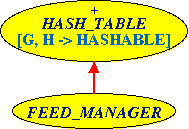
\includegraphics[scale=.6]{./figures/FEED_MANAGER}
  \caption{BON diagram of class \texttt{FEED\_MANAGER}}
  \label{fig:feed-manager}
\end{figure}


\section{Usage}
\label{sec:feed-manager-usage}

\begin{lstlisting}[language=Eiffel]
class
  FEED_MANAGER_EXAMPLE

create
  make

feature -- Initialization

  make is
      -- Creation procedure.
    do
      -- Create a simple feed
      create feed.make ("EiffelRSS", create {HTTP_URL}.make ("http://eiffelrss.berlios.de"), "EiffelRSS news")
      feed.set_refresh_period (15)
      feed.set_last_updated (create {DATE_TIME}.make_now)
      
      -- Add some simple items, use `feed.last_added_item' or directly create an item for finer control
      feed.new_item ("Version 23 released!", create {HTTP_URL}.make ("http://eiffelrss.berlios.de/Main/News"), "Version 23 of EiffelRSS got release today. Happy syndicating!")

      feed.new_item ("EiffelRSS wins award", create {HTTP_URL}.make ("http://eiffelrss.berlios.de/Main/Awards"), "EiffelRSS has been awarded by ISE as best syndication software written in Eiffel. For more info see award-winning pages: http://eiffelrss.berlios.de")

      -- Create feed manager
      create feed_manager.make
      feed_manager.add (feed, "http://eiffelrss.berlios.de/Main/AllRecentChanges?action=rss")
      feed_manager.refresh_all
    end
    
feature -- Arguments

  feed: FEED
      -- Example feed
      
  feed_manager: FEED_MANAGER
      -- Feed manager

end -- class FEED_MANAGER_EXAMPLE
\end{lstlisting}

\newpage

\section{Features}
\label{sec:feed-manager-features}

\subsection{Initialization}
\label{sec:feed-manager-initialization}

\subsubsection{make}

\begin{lstlisting}[language=Eiffel]
make
    -- Create a new feed manager with default refresh period `30'

\end{lstlisting}


\subsubsection{make\_custom}

\begin{lstlisting}[language=Eiffel]
make_custom (a_refresh_period: INTEGER)
    -- Create a new feed manager with default refresh period `a_refresh_period'
\end{lstlisting}


\subsection{Access}
\label{sec:feed-manager-access}

\subsubsection{default\_refresh\_period}

\begin{lstlisting}[language=Eiffel]
default_refresh_period: INTEGER
    -- Default refresh period in minutes
\end{lstlisting}

\subsubsection{last\_added\_feed}

\begin{lstlisting}[language=Eiffel]
last_added_feed: FEED
    -- feed that was last added
\end{lstlisting}

\subsubsection{feed\_addresses}

\begin{lstlisting}[language=Eiffel]
feed_addresses: LINKED_LIST[STRING]
    -- Returns a sortable list representation of the feeds saved in FEED_MANAGER
\end{lstlisting}

\subsubsection{feed\_links}

\begin{lstlisting}[language=Eiffel]
feed_links: LINKED_LIST[STRING]
    -- Returns a sortable list representation of the feeds saved in FEED_MANAGER
\end{lstlisting}


\subsection{Setter}
\label{sec:feed-manager-setter}

\subsubsection{set\_default\_refresh\_period}

\begin{lstlisting}[language=Eiffel]
set_default_refresh_period (a_refresh_period: INTEGER)
    -- Set refresh periode in minutes
\end{lstlisting}


\subsection{Element change}
\label{sec:feed-manager-element-change}

\subsubsection{add}

\begin{lstlisting}[language=Eiffel]
add (feed: FEED; url: STRING)
    -- Add `feed'
\end{lstlisting}

\subsubsection{add\_from\_url}

\begin{lstlisting}[language=Eiffel]
add_from_url (url: STRING)
    -- Add feed with URL `url'
\end{lstlisting}


\subsection{Refresh}
\label{sec:feed-manager-refresh}

\subsubsection{refresh}

\begin{lstlisting}[language=Eiffel]
refresh (url: STRING)
    -- Refresh feed with URL `url', if the feed is outdated
\end{lstlisting}

\subsubsection{refresh\_force}

\begin{lstlisting}[language=Eiffel]
refresh_force (url: STRING)
    -- Refresh feed with URL `url', even if the feed is not outdated
\end{lstlisting}

\subsubsection{refresh\_all}

\begin{lstlisting}[language=Eiffel]
refresh_all
    -- Refresh all feeds, if they are outdated
\end{lstlisting}

\subsubsection{refresh\_all\_force}

\begin{lstlisting}[language=Eiffel]
refresh_all_force
    -- Refresh all feeds, even if they are not outdated
\end{lstlisting}


\subsection{Conversion}
\label{sec:feed-manager-conversion}

\subsubsection{list\_representation}

\begin{lstlisting}[language=Eiffel]
list_representation: SORTABLE_TWO_WAY_LIST[FEED]
    -- Returns a sortable list representation of the feeds saved in FEED_MANAGER
\end{lstlisting}


\subsection{Conversion (sort)}
\label{sec:feed-manager-conversion-sort}

\subsubsection{sorted\_by\_last\_updated}

\begin{lstlisting}[language=Eiffel]
sorted_by_last_updated: SORTABLE_TWO_WAY_LIST[FEED]
    -- Returns a sorted list representation of the feeds, sorted by `last_updated'
\end{lstlisting}

\subsubsection{sorted\_by\_title}

\begin{lstlisting}[language=Eiffel]
sorted_by_title: SORTABLE_TWO_WAY_LIST[FEED]
    -- Returns a sorted list representation of the feeds, sorted by `title'
\end{lstlisting}

\subsubsection{sorted\_by\_link}

\begin{lstlisting}[language=Eiffel]
sorted_by_link: SORTABLE_TWO_WAY_LIST[FEED]
    -- Returns a sorted list representation of the feeds, sorted by `link'
\end{lstlisting}

\subsubsection{sorted\_by\_description}

\begin{lstlisting}[language=Eiffel]
sorted_by_description: SORTABLE_TWO_WAY_LIST[FEED]
    -- Returns a sorted list representation of the feeds, sorted by `description'
\end{lstlisting}

\subsubsection{reverse\_sorted\_by\_last\_updated}

\begin{lstlisting}[language=Eiffel]
reverse_sorted_by_last_updated: SORTABLE_TWO_WAY_LIST[FEED]
    -- Returns a sorted list representation of the feeds, reverse sorted by `last_updated'
\end{lstlisting}

\subsubsection{reverse\_sorted\_by\_title}

\begin{lstlisting}[language=Eiffel]
reverse_sorted_by_title: SORTABLE_TWO_WAY_LIST[FEED]
    -- Returns a sorted list representation of the feeds, reverse sorted by `title'
\end{lstlisting}

\subsubsection{reverse\_sorted\_by\_link}

\begin{lstlisting}[language=Eiffel]
reverse_sorted_by_link: SORTABLE_TWO_WAY_LIST[FEED]
    -- Returns a sorted list representation of the feeds, reverse sorted by `link'
\end{lstlisting}

\subsubsection{reverse\_sorted\_by\_description}

\begin{lstlisting}[language=Eiffel]
reverse_sorted_by_description: SORTABLE_TWO_WAY_LIST[FEED]
    -- Returns a sorted list representation of the feeds, reverse sorted by `description'
\end{lstlisting}


%-------------------------------------------------------------------------------
% Chapter: Class FEED_READER
%-------------------------------------------------------------------------------
\chapter{Class FEED\_READER}
\label{cha:feed-reader}

\section{Overview}
\label{sec:feed-reader-overview}

\texttt{FEED\_READER} is a helper class which manages everything to
load a feed.  It converts the data to an XML document object, detects
the format of the feed and uses the according reader object to convert
the XML document into a \texttt{FEED} object.

See figure \ref{fig:feed-reader} for an overview of the class.

\begin{figure}[htbp]
  \centering
  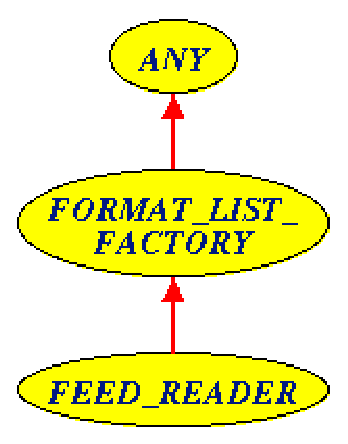
\includegraphics[scale=.6]{./figures/FEED_READER}
  \caption{BON diagram of class \texttt{FEED\_READER}}
  \label{fig:feed-reader}
\end{figure}


\section{Usage}
\label{sec:feed-reader-usage}

\begin{lstlisting}[language=Eiffel]
class
  READER_EXAMPLE

create
  make

feature -- Initialization

  make is
      -- Creation procedure.
    local
      location: STRING
      reader: FEED_READER
      feed: FEED
    do
      -- Get a feed location from the user
      io.put_string ("Enter an URL: ")
      io.read_line
      
      location := io.last_string.twin
      
      -- Create the reader
      create reader.make_url (location)
      
      -- Get the feed
      feed := reader.read
      
      -- Print feed
      io.put_string ("%NReceived feed:%N")
      io.put_string ("==============%N%N%N")
      io.put_string (feed.to_string)
    end

end -- class READER_EXAMPLE
\end{lstlisting}


\section{Features}
\label{sec:feed-reader-features}

\subsection{Initialization}
\label{sec:feed-reader-initialization}

\subsubsection{make\_url}

\begin{lstlisting}[language=Eiffel]
make_url (a_url: STRING)
  -- Create with `a_url' as source of feed
\end{lstlisting}


\subsection{Basic operations}
\label{sec:feed-reader-basic-operations}

\subsubsection{read}

\begin{lstlisting}[language=Eiffel]
read: FEED
  -- Load the data from the given url into a FEED
\end{lstlisting}


%-------------------------------------------------------------------------------
% Chapter: Class FEED_WRITER
%-------------------------------------------------------------------------------
\chapter{Class FEED\_WRITER}
\label{cha:feed-writer}

\section{Overview}
\label{sec:feed-writer-overview}

\texttt{FEED\_WRITER} is a helper class which manages everything to
write a feed. It converts the data from an existing \texttt{FEED}
object into an XML document object and saves it into a local file.


\section{Usage}
\label{sec:feed-writer-usage}

\begin{lstlisting}[language=Eiffel]
class
  WRITER_EXAMPLE

create
  make

feature -- Initialization

  make is
      -- Creation procedure.
  local
      feed: FEED
      writer: FEED_WRITER
  do
      -- Create a simple feed
      create feed.make ("EiffelRSS", create {HTTP_URL}.make ("http://eiffelrss.berlios.de/Main/AllRecentChanges?action=rss"), "EiffelRSS news")
      
      -- Add some simple items
      feed.new_item ("Version 23 released!", create {HTTP_URL}.make ("http://eiffelrss.berlios.de/Main/News"), "Version 23 of EiffelRSS got release today. Happy syndicating!")      
      feed.new_item ("Microsoft uses EiffelRSS", create {HTTP_URL}.make ("http://eiffelrss.berlios.de/Main/WhoUsesEiffelRSS"), "Microsoft announced in a press release today that they will use EiffelRSS to syndicate news on their website.")
      feed.new_item ("EiffelRSS wins award", create {HTTP_URL}.make ("http://eiffelrss.berlios.de/Main/Awards"), "EiffelRSS has been awarded by ISE as best syndication software written in Eiffel. For more info see award-winning pages: http://eiffelrss.berlios.de")
        
      -- Write feed to file
      create writer.make_feed (feed)
      writer.write ("example.xml", "RSS 2.0")
  end

end -- class WRITER_EXAMPLE
\end{lstlisting}


\section{Features}
\label{sec:feed-writer-features}

\subsection{Initialization}
\label{sec:feed-writer-initialization}

\subsubsection{make\_feed}

\begin{lstlisting}[language=Eiffel]
make_feed (a_feed: FEED) is
  -- Create a writer object for the feed `a_feed'
\end{lstlisting}


\subsection{Basic operations}
\label{sec:feed-writer-basic-operations}

\subsubsection{write}

\begin{lstlisting}[language=Eiffel]
write (a_filename, a_format: STRING) is
  -- Write the feed to a local file with `a_filename' in the format `a_format'
  -- You can enumerate all available formats with FORMAT_LIST (see FORMATS)
\end{lstlisting}